\documentclass{article}

\usepackage{graphicx}
\usepackage{multirow}
\usepackage{amsmath,amssymb,amsfonts,amsthm, mathrsfs}
\usepackage[title]{appendix}
\usepackage{xcolor}
\usepackage{textcomp}
\usepackage{manyfoot, booktabs}
\usepackage{algorithm, algorithmicx, algpseudocode}
\usepackage{listings}
\usepackage{biblatex}

\usepackage[english]{babel}

\raggedbottom

\lstset{
    language=Python,                 
    basicstyle=\ttfamily\small,      
    keywordstyle=\color{blue},       
    stringstyle=\color{red},         
    commentstyle=\color{orange},      
    morecomment=[s][\color{gray}]{"""}{"""}, 
    numbers=left,                    
    numberstyle=\tiny\color{gray},   
    stepnumber=1,                    
    numbersep=10pt,                  
    backgroundcolor=\color{white},   
    showspaces=false,                
    showstringspaces=false,          
    showtabs=false,                  
    frame=single,                    
    captionpos=b,                    
    breaklines=true,                 
    breakatwhitespace=false,         
    tabsize=4,                       
    escapeinside={\%*}{*}           
}

\begin{document}

\title{F1 EDA - Big Data Final Term Project}

\author{Enrique Ulises Báez Gómez Tagle \\ Mauricio Iván Ascencio Martínez\\ Sara Rocío Miranda Mateos}

\maketitle

\begin{abstract}
In this project, we explore the use of big data technologies to analyze the Formula 1 dataset. Our objective is to derive meaningful insights that can inform strategic decisions in the sport.
\end{abstract}

\tableofcontents
\newpage

\section{Introduction}
This project focuses on leveraging big data technologies to analyze the Formula 1 dataset. By implementing a robust data lakehouse architecture, we aim to perform detailed data analysis and extract insights that can drive data-driven decision-making in the context of Formula 1 racing.

\section{Infrastructure / Architecture}

\begin{itemize}
    \item \textbf{Data Lakehouse Configuration:} Central to our project is a Data Lakehouse architecture designed for scalability and resilience within an AWS environment. This setup includes multiple layers of data storage and processing capabilities, ensuring efficient data management and analysis.
    
    \item \textbf{Storage Layers:} 
        \begin{itemize}
            \item \textbf{Raw Data Storage (RAW Layer):} Utilizes Amazon S3 to store unprocessed, raw data ingested from various sources.
            \item \textbf{Cleansed Data Storage (Cleansed Layer):} Stores cleaned and transformed data in Amazon S3, ready for further analysis.
            \item \textbf{Data Warehouse Storage (Data Warehouse Layer):} Contains structured and optimized data in Amazon S3, prepared for querying and visualization.
        \end{itemize}
    
    \item \textbf{Data Ingestion:} 
        \begin{itemize}
            \item \textbf{Real-Time Data Ingestion (AWS Lambda):} Handles the real-time ingestion of data, storing it in the RAW Layer.
            \item \textbf{Batch Data Ingestion (Static Dataset):} Manages the batch ingestion of static datasets, such as CSV files, into the RAW Layer.
        \end{itemize}
    
    \item \textbf{Data Transformation:} 
        \begin{itemize}
            \item \textbf{ETL Processing Jobs (AWS Glue):} Performs ETL (Extract, Transform, Load) operations to clean and transform data from the RAW Layer to the Cleansed Layer.
        \end{itemize}
    
    \item \textbf{Data Analysis:} 
        \begin{itemize}
            \item \textbf{Data Analytics and Processing (AWS EMR):} Utilizes Amazon EMR to run advanced data processing and analytical tasks on data from the Cleansed Layer, producing structured results stored in the Data Warehouse Layer.
        \end{itemize}
    
    \item \textbf{Data Cataloging:} 
        \begin{itemize}
            \item \textbf{Metadata Management (AWS Glue Data Catalog):} Catalogs the metadata of datasets in the Cleansed Layer, facilitating efficient data discovery and access.
        \end{itemize}
    
    \item \textbf{Data Visualization:} 
        \begin{itemize}
            \item \textbf{Visualization and Analysis (RStudio):} Processes the curated datasets in the Data Warehouse Layer locally to create insightful visualizations and analysis, supporting decision-making.
        \end{itemize}
    
    \item \textbf{Deployment Process:}
        \begin{enumerate}
            \item We initiated our deployment by setting up the AWS CLI, enabling us to interact with AWS services seamlessly.
            \item Amazon S3 buckets were created to host our data layers, carefully chosen to be in proximity to our compute resources to minimize latency.
            \item For infrastructure provisioning, we utilized both AWS CloudFormation and Terraform. AWS CloudFormation was used for managing AWS-specific resources, ensuring consistent and repeatable deployments within the AWS ecosystem. Terraform was employed for managing multi-cloud resources and ensuring infrastructure as code principles across various environments.
            \item AWS Glue was configured to automate our ETL processes, facilitating efficient data transformation and loading into our cleansed and data warehouse layers.
            \item Amazon EMR clusters were set up for big data processing, with configurations tailored to optimize performance and cost.
            \item Continuous Integration and Continuous Deployment (CI/CD) pipelines were implemented using AWS CodePipeline and Jenkins, automating the deployment process and ensuring that updates to our infrastructure and applications could be rolled out smoothly.
            \item Monitoring and logging were established using Amazon CloudWatch and AWS CloudTrail, providing real-time insights and audit trails for all activities within our environment.
            \item Security best practices were followed, including the use of IAM roles and policies to control access, as well as encryption of data at rest and in transit to protect our sensitive information.
        \end{enumerate}
    
\end{itemize}

This infrastructure is pivotal to our project, allowing us to effectively utilize big data technologies to derive valuable insights from the Formula 1 dataset. The design prioritizes scalability, efficiency, and cost-effectiveness, ensuring it meets the high demands of large-scale data processing and analysis. Ultimately, this setup empowers us to make data-driven decisions that enhance our understanding and strategic planning within the context of Formula 1.

\begin{figure}[H]
    \centering
    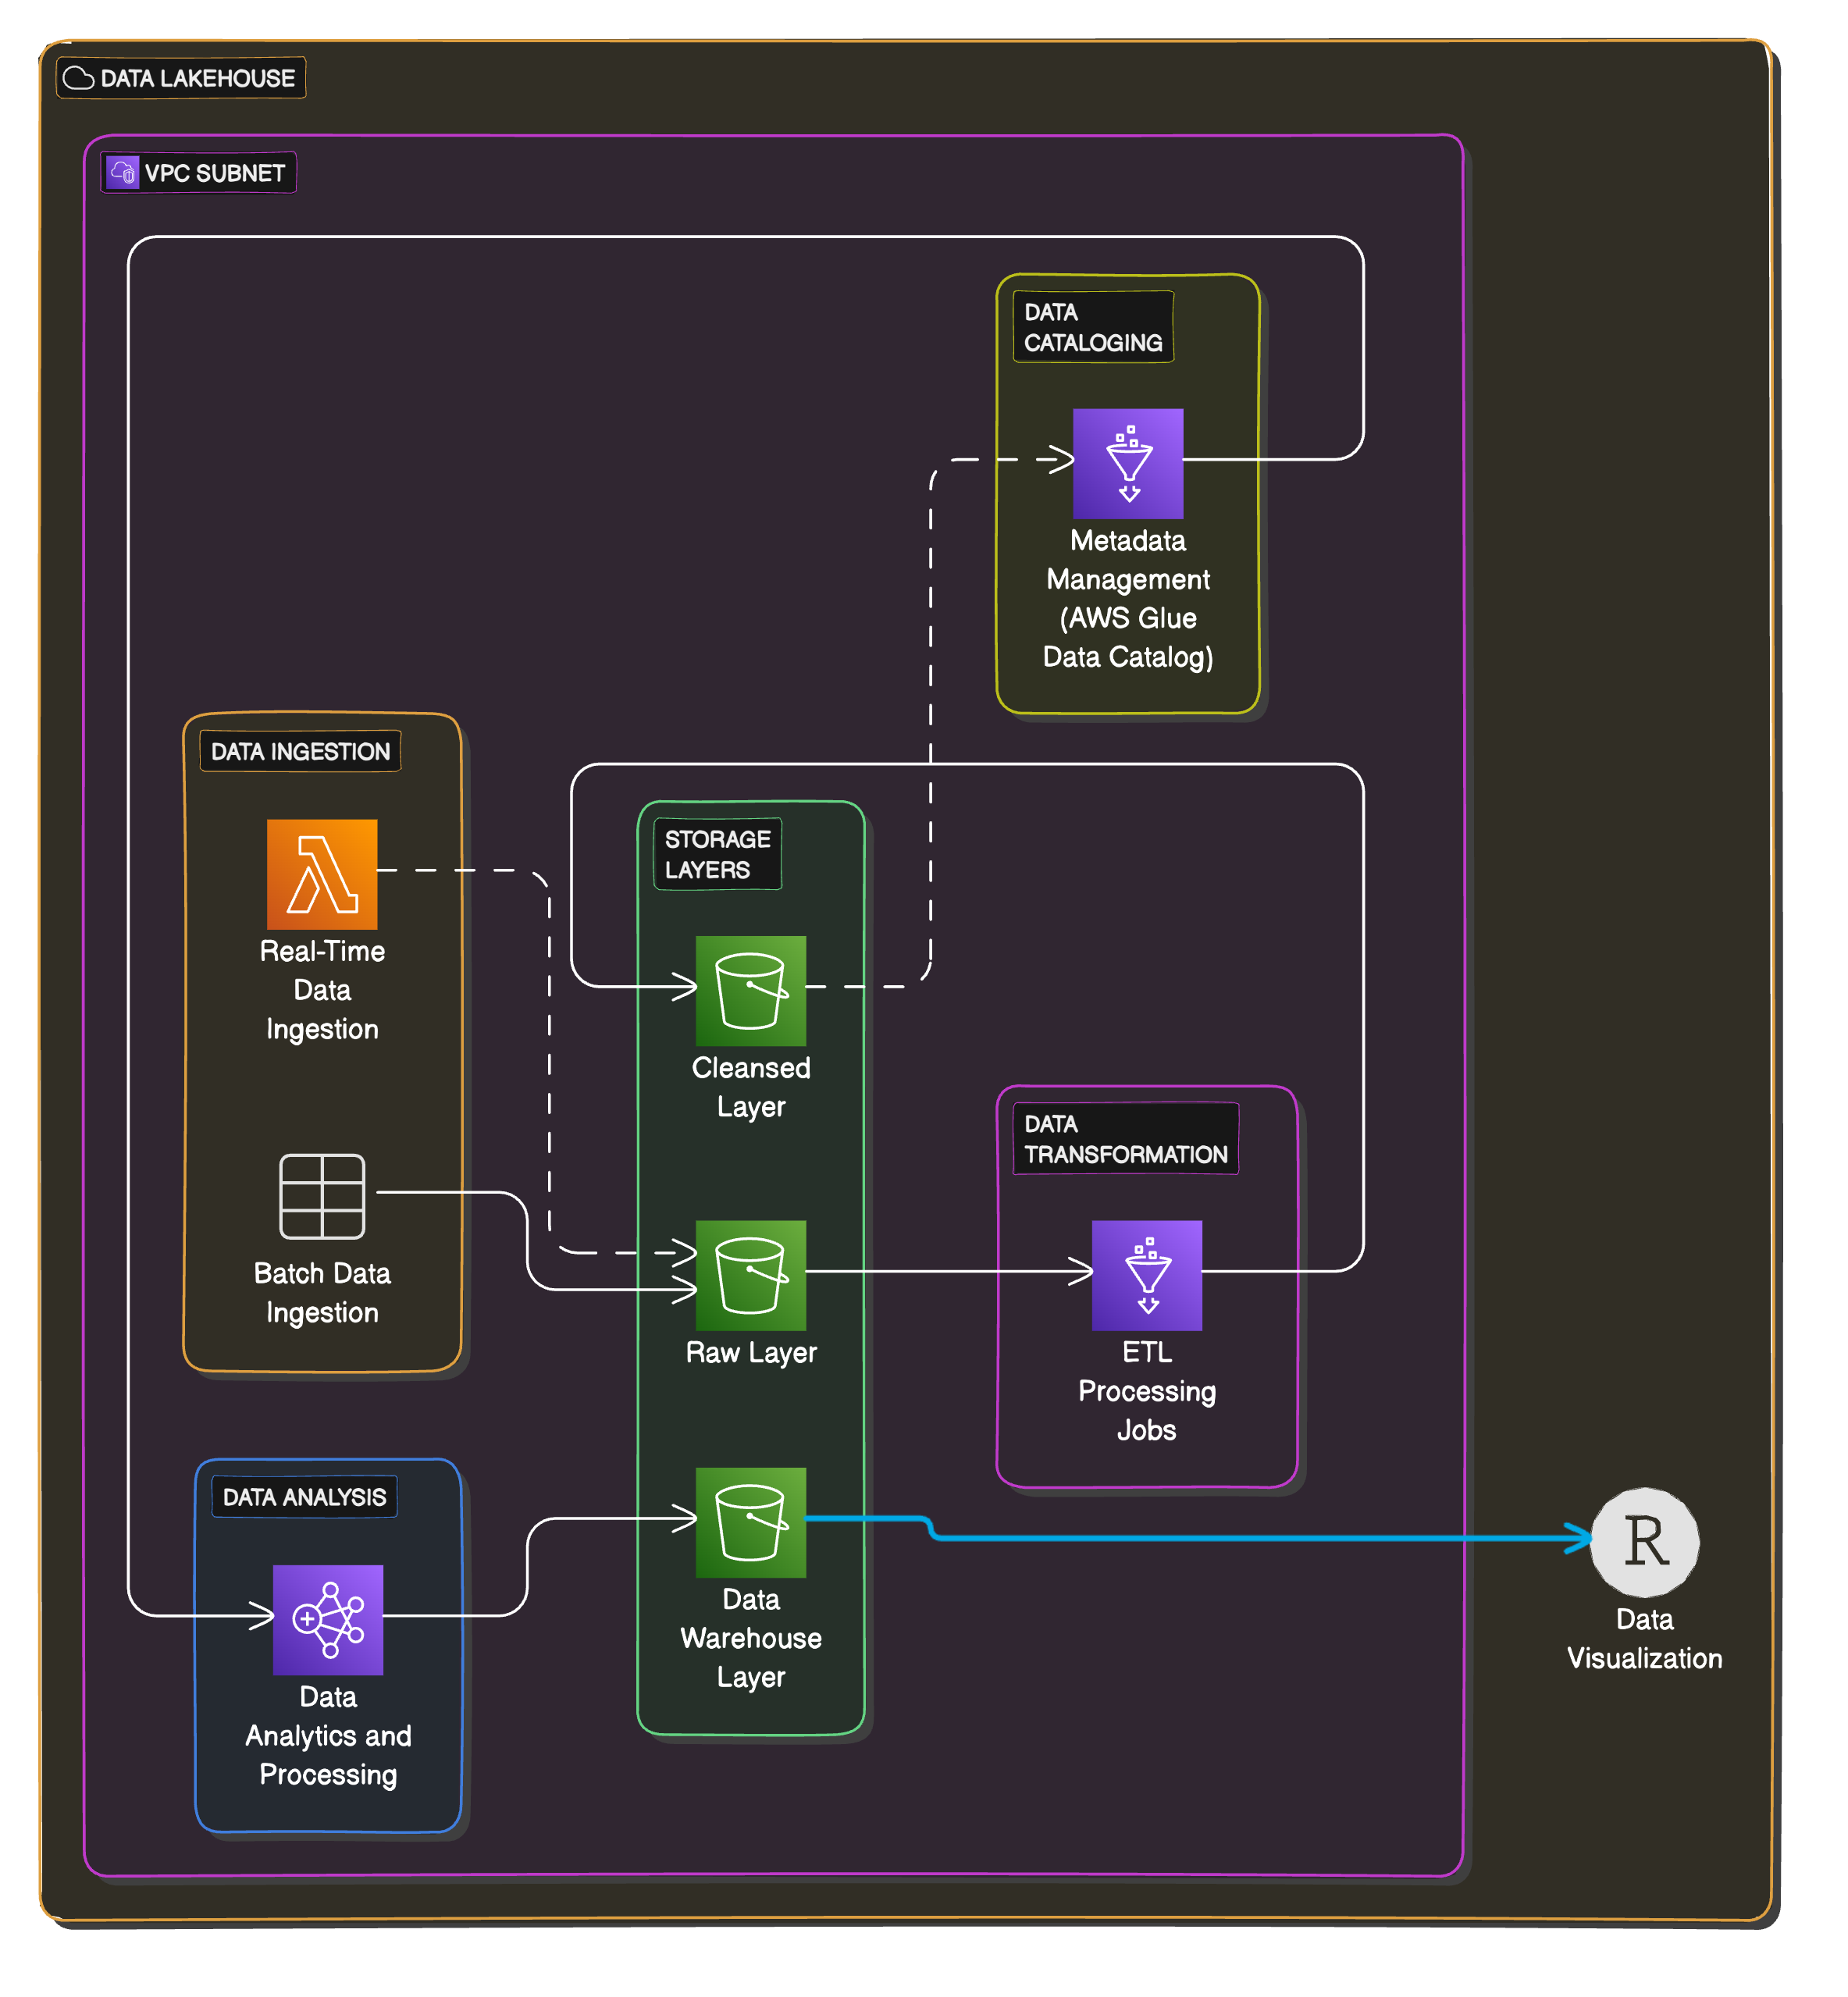
\includegraphics[width=0.7\textwidth]{images/arch/AWS-GridGuru-LakeHouseArchitecture.png}
    \caption{\textbf{Architecture Diagram}}
\end{figure}

\section{Data Analysis with F1 Dataset}

\begin{lstlisting}[language=Python]
# Placeholder for Python code
\end{lstlisting}

\subsection{Query Analysis and Insights}

\subsubsection{Average Number of Laps per Grand Prix}
\paragraph{Description:}
The average number of laps per Grand Prix provides insights into race length and potential strategy implications for teams.

\begin{figure}[H]
    \centering
    %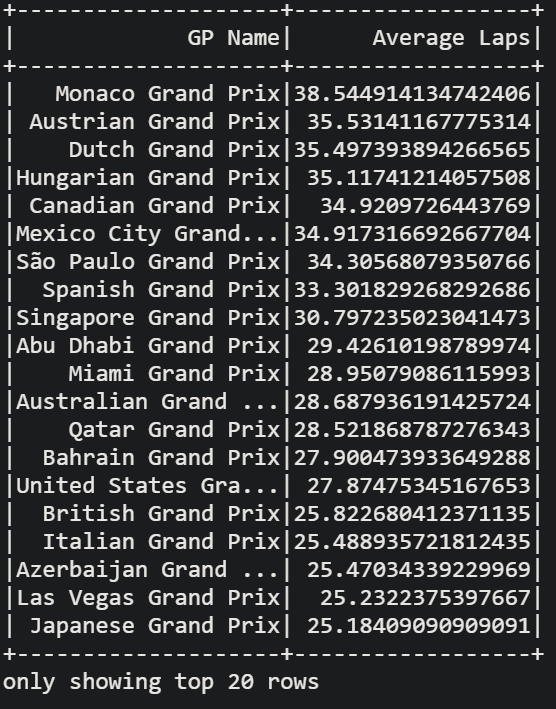
\includegraphics[width=0.6\textwidth]{ss-average-laps.png}
    \caption{Number of Laps GCP Query Result}
\end{figure}

\begin{figure}[H]
    \centering
    %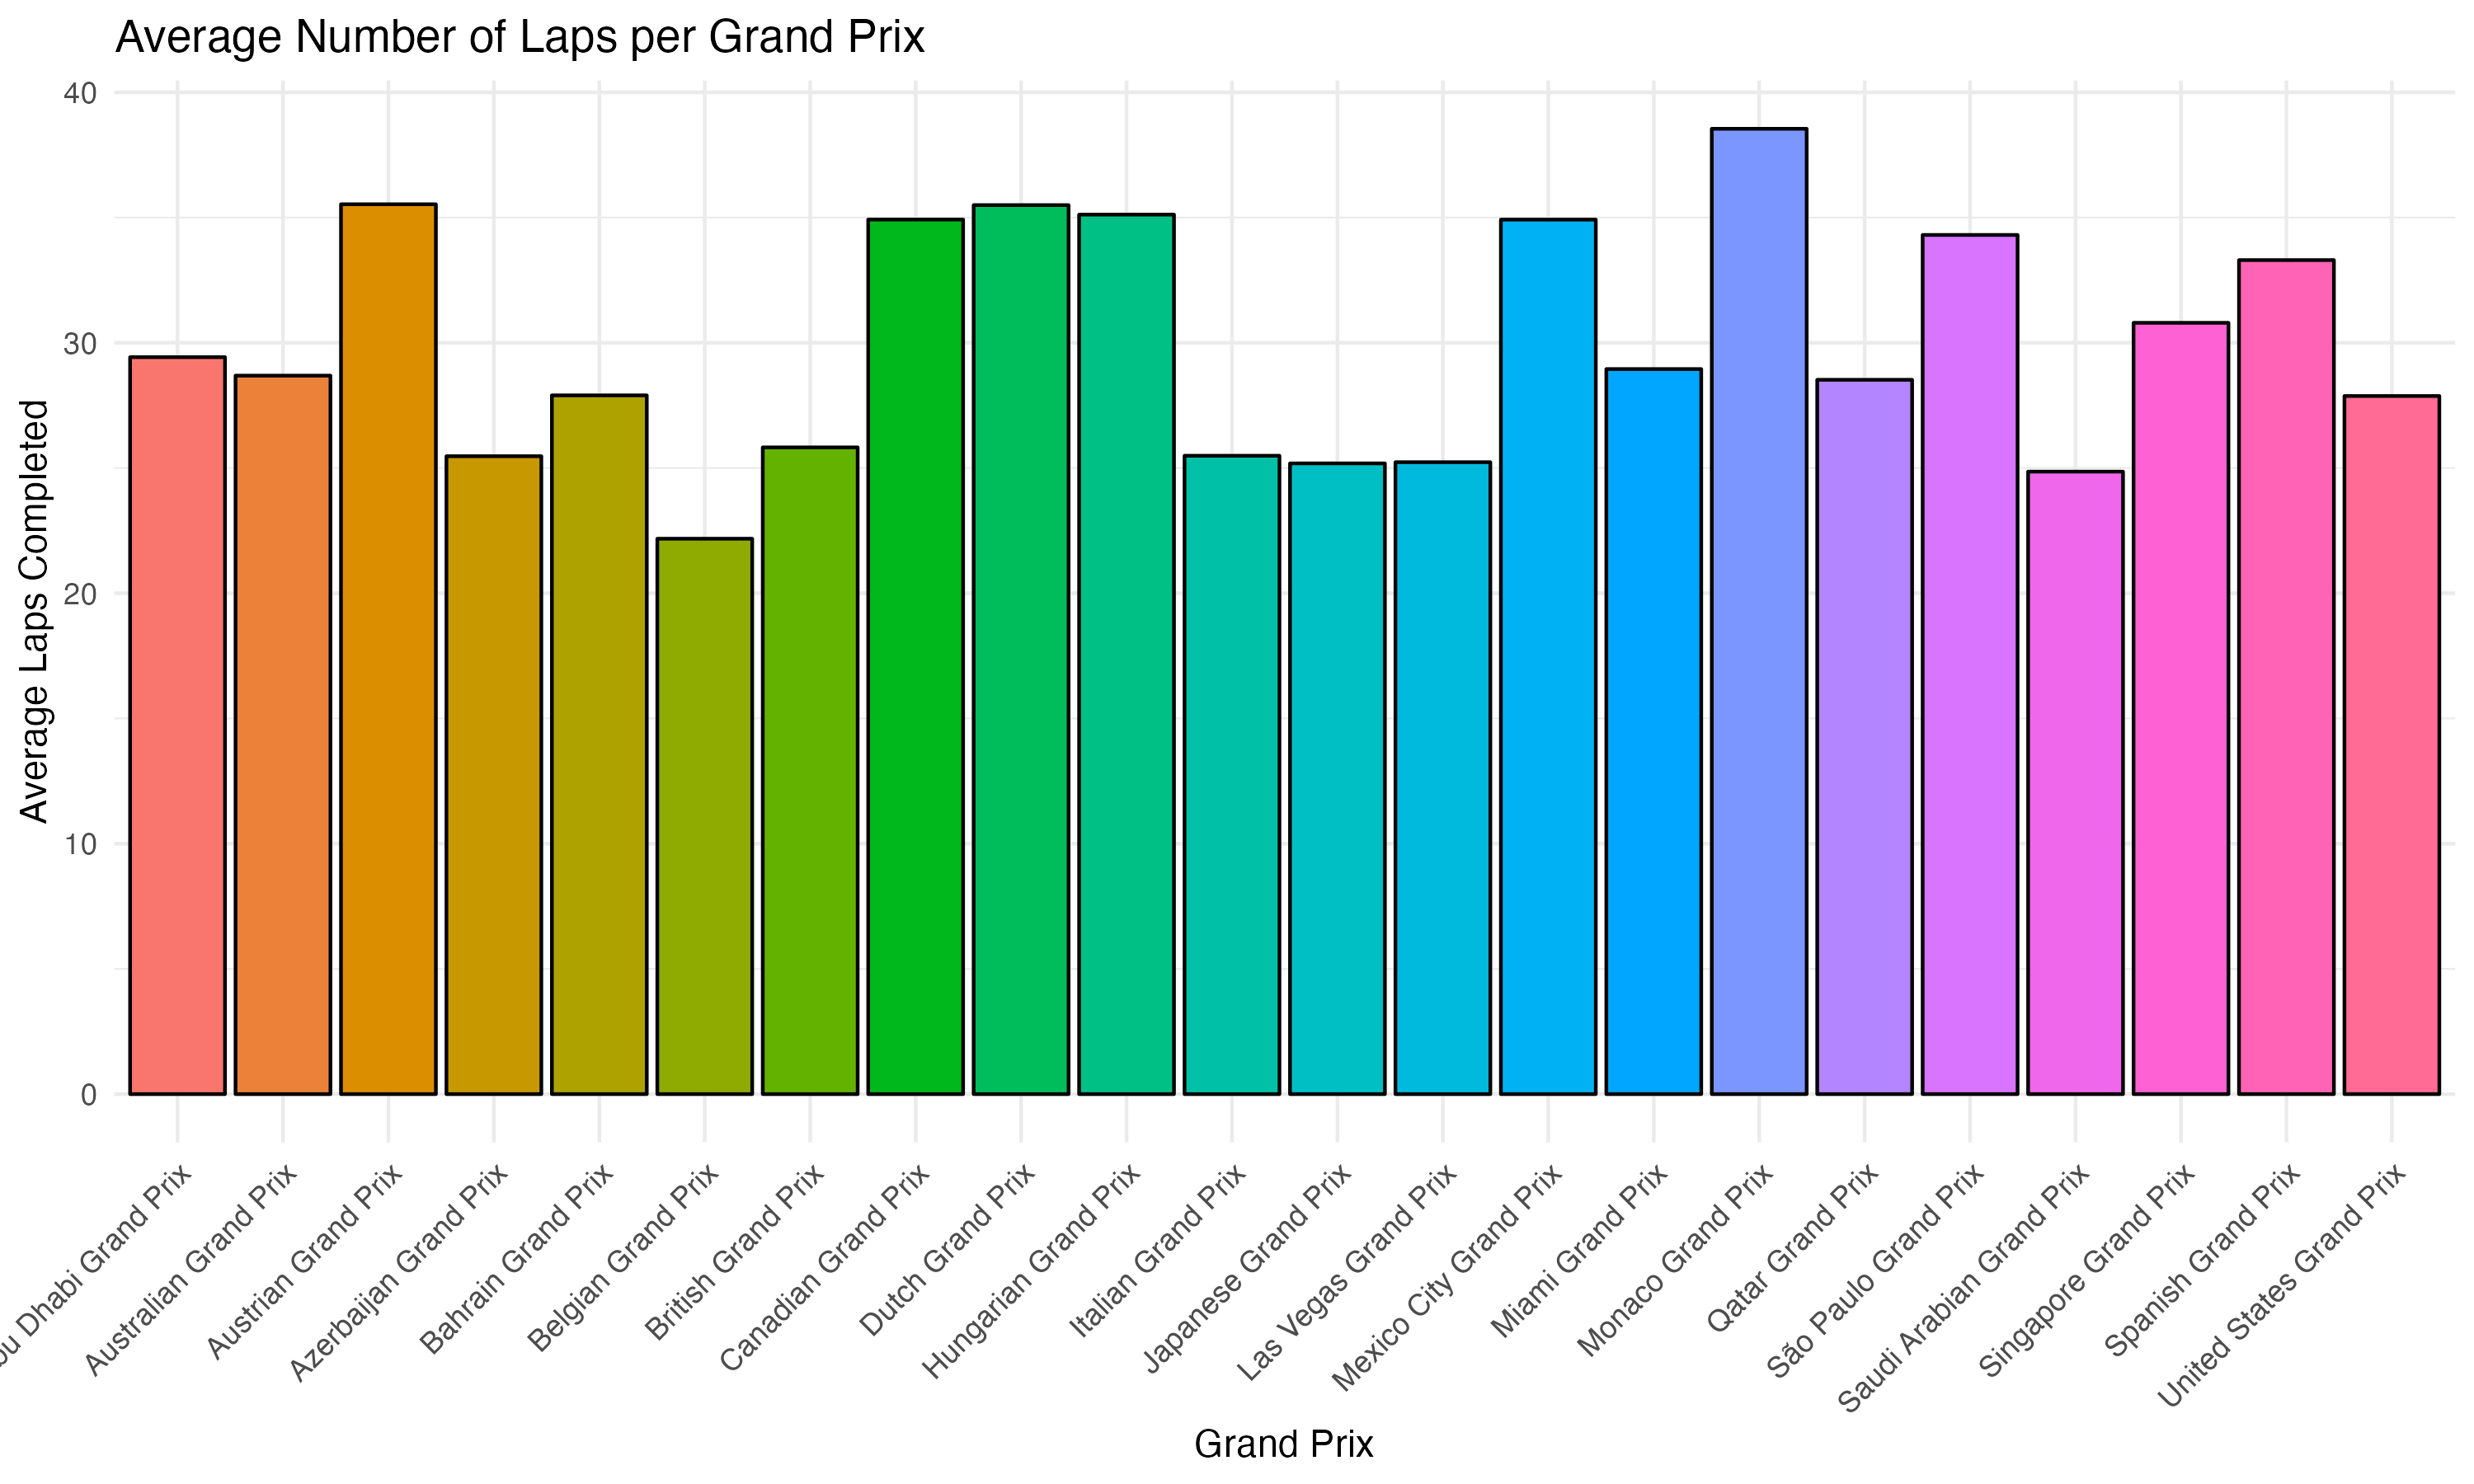
\includegraphics[width=\textwidth]{average_laps_per_gp_plot.png}
    \caption{Bar Chart Average Number of Laps per Grand Prix}
\end{figure}

\paragraph{Interpretation:}
The bar graph visually represents the average number of laps for each Grand Prix, sorted in descending order. Longer races may indicate a need for different tire strategies or fuel management plans. Conversely, shorter races might lead to more aggressive racing tactics. We can say that Monaco GP is the longest and Belgian GP is the shortest with a difference of around 16 laps.

\section{Challenges Encountered}
During the development and analysis phases of our project, we encountered several challenges that fell into two main categories: infrastructure-related and query/code-related. Below, we detail these issues and how we addressed them.

\subsection{Infrastructure-Related Challenges}
\paragraph{Description:}
Some of the challenges faced were related to the setup and configuration of the AWS services, ensuring efficient data flow between different layers, and maintaining security and compliance standards.

\subsection{Query and Code-Related Challenges}
\paragraph{Description:}
Challenges included optimizing queries to handle large datasets efficiently and debugging code to ensure accurate analysis results.

\section{Conclusions}
Through the utilization of big data technologies such as AWS and the implementation of a robust data lakehouse architecture, this project has provided significant insights into the Formula 1 dataset. Our comprehensive analysis spanned multiple aspects of the sport, from individual driver performance and tire strategies to the influence of weather conditions on race dynamics.

\paragraph{Insights and Impact:}
The queries conducted revealed:
\begin{itemize}
    \item Insights into race strategies based on the number of laps per Grand Prix.
    \item Data-driven decisions for tire management and fuel strategies.
\end{itemize}

\paragraph{Future Directions:}
Future work could involve incorporating additional data sources, such as weather data, to enhance the analysis and insights.

\paragraph{Final Thoughts:}
This project demonstrates the power of big data technologies in sports analytics, providing a framework for future analysis and strategic planning in Formula 1.

\section{Project Repository}
\url{https://github.com/enriquegomeztagle/BigData/tree/main/FinalTerm/F1-GridGuru-Project}

\section{References}
\label{sec:references}
\begin{thebibliography}{9}
\bibitem{ref1}
Author, \textit{Title of the paper}, Journal Name, Volume, Year.
\end{thebibliography}

\end{document}
